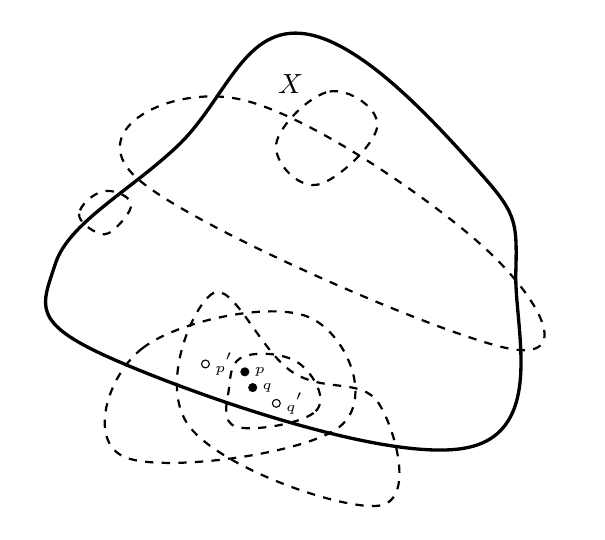
\begin{tikzpicture}

\draw [very thick] plot[smooth cycle, tension=.7] coordinates {(-4.107,4.0707) (-2.5611,5.562) (-1,7) (1.2182,5.305) (1.7413,3.9553) (1.1256,1.7374)   (-3.4205,2.8821) };

\coordinate (S) at (-1.4,6.6) {};
\node[{anchor=north west }] at (S){$X$};

\draw [thick,dashed]  plot[smooth cycle, tension=.7] coordinates {(-1.1,2.7) (-2.1,3.7) (-2.4,2)(0,1) (0,2.3) };
\draw [ thick,dashed]  plot[smooth cycle, tension=.7] coordinates {(-0.9,3.4) (-3,3) (-3.2162,1.6137)  (-0.5,2) };
\draw [ thick,dashed]  plot[smooth cycle, tension=.7] coordinates {(-1.8,2) (-0.8,2.2) (-1,2.8)(-1.7,2.9)  (-1.9,2.5) };



\draw [thick,dashed]  plot[smooth cycle, tension=.7] coordinates {(-3.502,4.9926) (-3.8054,4.708) (-3.5483,4.4576)(-3.3207,4.5465) (-3.1499,4.8536) };
\draw [ thick,dashed]  plot[smooth cycle, tension=.7] coordinates {(-1.7736,6.1636) (1.3735,4.2485) (1.6328,3.0001)  (-3.0857,5.1744) };
\draw [ thick,dashed]  plot[smooth cycle, tension=.7] coordinates {(-1.3019,5.5919) (-0.6223,6.2606) (-0.0187,5.8136)  (-0.7827,5.0761) };


\coordinate (N2) at (-1.6,2.5) {} {} {} {} {} {} {};
\node[right] at (N2){\tiny$q$};;
\draw[fill=black]  (N2) circle (0.05);

\coordinate (p1) at (-1.7,2.7) {} {} {} {} {} {} {};
\node[right] at (p1){\tiny$p$};;
\draw[fill=black]  (p1) circle (0.05);
\coordinate (p2) at (-2.2,2.8) {} {} {} {} {} {};
\node[right] at (p2){\tiny$p^{'}$};;
\draw[fill=white]  (p2) circle (0.05);
\coordinate (N) at (-1.3,2.3) {} {} {} {} {} {} {};
\draw[fill=white]  (N) circle (0.05);
\node[right] at (N){\tiny$q^{'}$};

%\coordinate (L) at (-0.6,0.2) {} {} {} {};
%\node[right] at (L){\tiny$A_i$};;
%\draw[-{Latex[length=2mm]}]  plot[smooth, tension=.7] coordinates {(L) (0,-0.5)(-0.3,-0.4) (-0.5,0.5)};
%\coordinate (L2) at (-16.5,-0.5) {} {} {} {} {} {};
%\node[below] at (L2){\tiny$B_i= U\cup (U\cap A_i)$};;
%\draw[-{Latex[length=2mm]}]  plot[smooth, tension=.7] coordinates {(L2) (-12.5,1)(-11,2) (-8,3)};
\end{tikzpicture}
